\title{Markov chains and their computation}
\author{Gavin Pownall}
\documentclass[12pt]{article}

\usepackage{amsmath}
\usepackage{tikz}
\usetikzlibrary{automata, positioning}

\begin{document}
\maketitle

\begin{abstract}
The following decribes what a Markov chain is and how the state of a Markov Chain system is computed at any time step.
\end{abstract}

\section{Markov Chain computation}
A Markov chain is ``a stochastic model desribing a sequence of events in which the probability of an event depends only on the state attained in the previous event'' (see Wikipedia). 
This is explained with an example such as the one below.

Say that there are three possible states you can hold: $A$, $B$ and $C$. If you are in $A$, the probability of moving from $A$ to $B$ is $M_{B,A}$, if you are in $C$ the probability of moving to $A$ is $M_{A,C}$. For any state $i$, the probability of staying in that same position for the next measurement is $M_{i,i}$. Etc. An example is given in Fig. \ref{fig:markov_chain}.

The probabilities can be represented by a \emph{stochastic} matrix $M_{i,j}$, where $(A, B, C)$ maps to $(1, 2, 3)$. For Fig. \ref{fig:markov_chain}, we have the following matrix:

\begin{equation}
	\begin{pmatrix}
		1/3 & 1/2 & 1/10\\
		1/3 & 1/4 & 2/10\\
		1/3 & 1/4 & 7/10
	\end{pmatrix}
\end{equation}

Notice how, for each column, the elements total one.

\begin{figure} \label{fig:markov_chain}
\centering
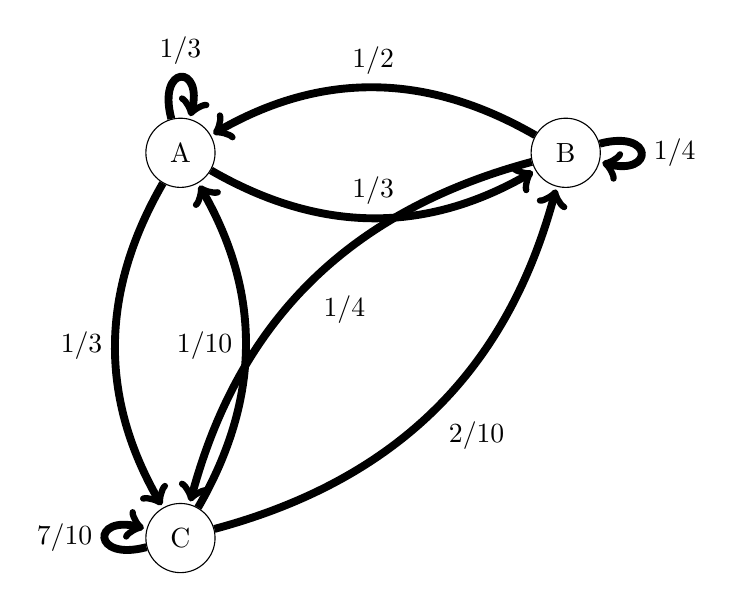
\begin{tikzpicture}
    \node[state] (A) {A};
    \node[state, right=4cm of A] (B) {B};
    \node[state, below=4cm of A] (C) {C};
	\draw[every loop, line width=1mm]
	    (A) edge[bend right, auto=left] node {1/3} (B)
	    (A) edge[bend right, auto=right] node {1/3} (C)
            (A) edge[loop above] node {1/3} (A)
	    (B) edge[bend right, auto=right] node {1/2} (A)
	    (B) edge[bend right, auto=left] node {1/4} (C)
	    (B) edge[loop right] node {1/4} (B)
	    (C) edge[bend right, auto=left] node {1/10} (A)
	    (C) edge[bend right, auto=right] node {2/10} (B)
	    (C) edge[loop left] node {7/10} (C);
\end{tikzpicture}
	\caption{A display of a 3-state Markov-chain process.}
\end{figure}

We also need to define an initial state $I$, which will simply be the probability of being in each state at time step $0$, for example $(1/3, 1/3, 1/3)$ or $(1, 0, 0)$. 
Again, this must sum to one.
We label this $P_0$.

The probability of being in any step at time $t$ is 
\begin{equation}
	P_{t} = MP_{t-1}
\end{equation}

In other words, by the definition that this is a Markov-chain process, the probability matrix is multiplied by the previous state in order to give the current state.
Given $P_0$ and $M$, we can therefore calculate the probability of the state at any time $t$ in one line:

\begin{equation}
	P_{t} = M^t P_{0}
\end{equation}

Obviously this isn't ideal to do by hand, and even for a computer this could get expensive for a large number of states or large values of $t$. For this reason, we diagonalise the $M$ matrix -- or, in simpler terms, express $P_0$ in terms of the eigenvectors of $M$. 

Define the eigenvalues of $M$ to be $m_i$ and the eigenvectors to be $e_i$. 
The initial state is written in terms of the eigenvectors to give:

\begin{equation}
	\begin{aligned}
		P_{t} &= M^t P_{0}\\
		&= \sum_{n=1}^{i} M^t c_n e_n\\
		&= \sum_{n=1}^{i} c_n m_n^t e_n,
	\end{aligned}
\end{equation}
where $c_i$ are scalar values, $P_{0} = \sum_{n=1}^{i} c_n e_n$.
This is far faster to compute.

Notes:
\begin{itemize}
	\item It is given without proof that the eigenvectors of a stochastic matrix span the full space they inhabit.
	\item It is given, again without proof, that one of the eigenvalues is $1$ and that the others are less than $1$. As a result, clearly from the above equation, as $t\rightarrow \infty$, all of the terms in the sum vanish except for one. This is known as the \emph{stationary state}.
\end{itemize}

\section{Python code}
The class for computing all of the above is given in MarkovClass.py.
By running this script directly, the above example is computed.
\begin{verbatim}
python3 MarkovClass.py

Initial state:  [1 0 0]
Probability matrix:
  [[0.33333333 0.5        0.1       ]
 [0.33333333 0.25       0.2       ]
 [0.33333333 0.25       0.7       ]]
Constants:  [ 0.49382716 -0.42910033  0.43247949]
Eigenvalues:  [ 1.          0.39013419 -0.10680086]
Eigenvectors:  [[ 0.525       0.5         1.        ]
 [-0.7183897  -0.2816103   1.        ]
 [ 1.         -0.85033548 -0.14966452]]
Equation with time:
P(t) = 0.4938271604938267*(1.0000000000000009^t)*[0.525 0.5   1.   ] 
+-0.42910032543113297*(0.39013419193125953^t)*[-0.7183897 -0.2816103  1.       ] 
+0.43247948804680914*(-0.10680085859792622^t)*[ 1.         -0.85033548 -0.14966452]
Stationary state: [0.25925926 0.24691358 0.49382716]
\end{verbatim}

There are clearly issues with floating point errors, but these come directly from the numpy linear algebra computation and unfortunately cannot be helped.

\section{Example usages}

Python scripts are available for both of the below examples, as well as gifs showing the state over time.

\subsection{Gambler's ruin}

The Gambler's ruin problem is well known. 
Given a starting value, x, a value at which the gambler would ``cash out'', y, and a probability of increasing by 1 and decreasing by 1, what is the probability that the gambler would eventually cash out?

This can be solved using an iterative derivation. For example, for a fair coin the probability of ending penniless is:
\begin{equation}
	P = \frac{x}{y}.
\end{equation}
Using Markov chains, not only can this be calculated computationally, but you can also calculate the probability of the gambler having a certain number of coins at any time step. See GamblersRuin.py for more details.

\subsection{Monopoly}

The monopoly game can also be simulated using Markov chain analysis. In the Monopoly.py script, a simple setup is created with dice rolls and chance/community chest ``advance to'' cards accounted for. The stationary state gives the optimal position for properties. 
As has been observed elsewhere, the jail square is the most likely, followed by those around 7 squared afterward.
The stationary state of the monopoly board is visualised in Fig. \ref{fig:monopoly}.

\begin{figure}\label{fig:monopoly}
	\centering
	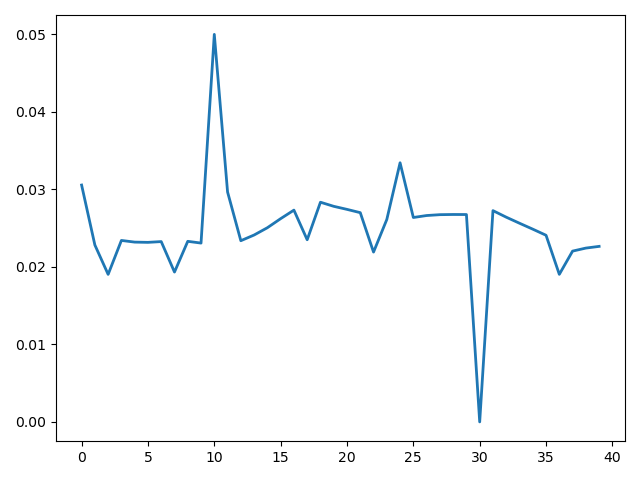
\includegraphics[width=0.6\textwidth]{MonopolyStationary.png}
\end{figure}

\end{document}
